\subsection{\textcolor{Salmon}{Ergebnisse Usability Test}}
\textcolor{blue}{\textit{einleitende Worte}}\\

\noindent
\underline{Fehlerbetrachtung}\\
- Fehlende Daten aus Gründen xy\\

\noindent
\underline{Genauigkeit-Zeit-Vergleich}\\

\noindent
\underline{s. \autoref{tab:usability_test:mittelwerte}}\\
- Differenz berechnen, Fehlerquote als Wert\\
-> Berechnung Fehlerquote in Tabelle im Anhang \autoref{fig:Usability-Test:Excel_Berechnungen}\\
- grafisch dargestellt in \autoref{fig:usability_test:genauigkeit-zeit_alt-neu} \&\& \autoref{fig:usability_test:genauigkeit-zeit_alle-richtige}

%\subsection{Genauigkeit-Zeit}
\begin{figure}[H]
    \centering
    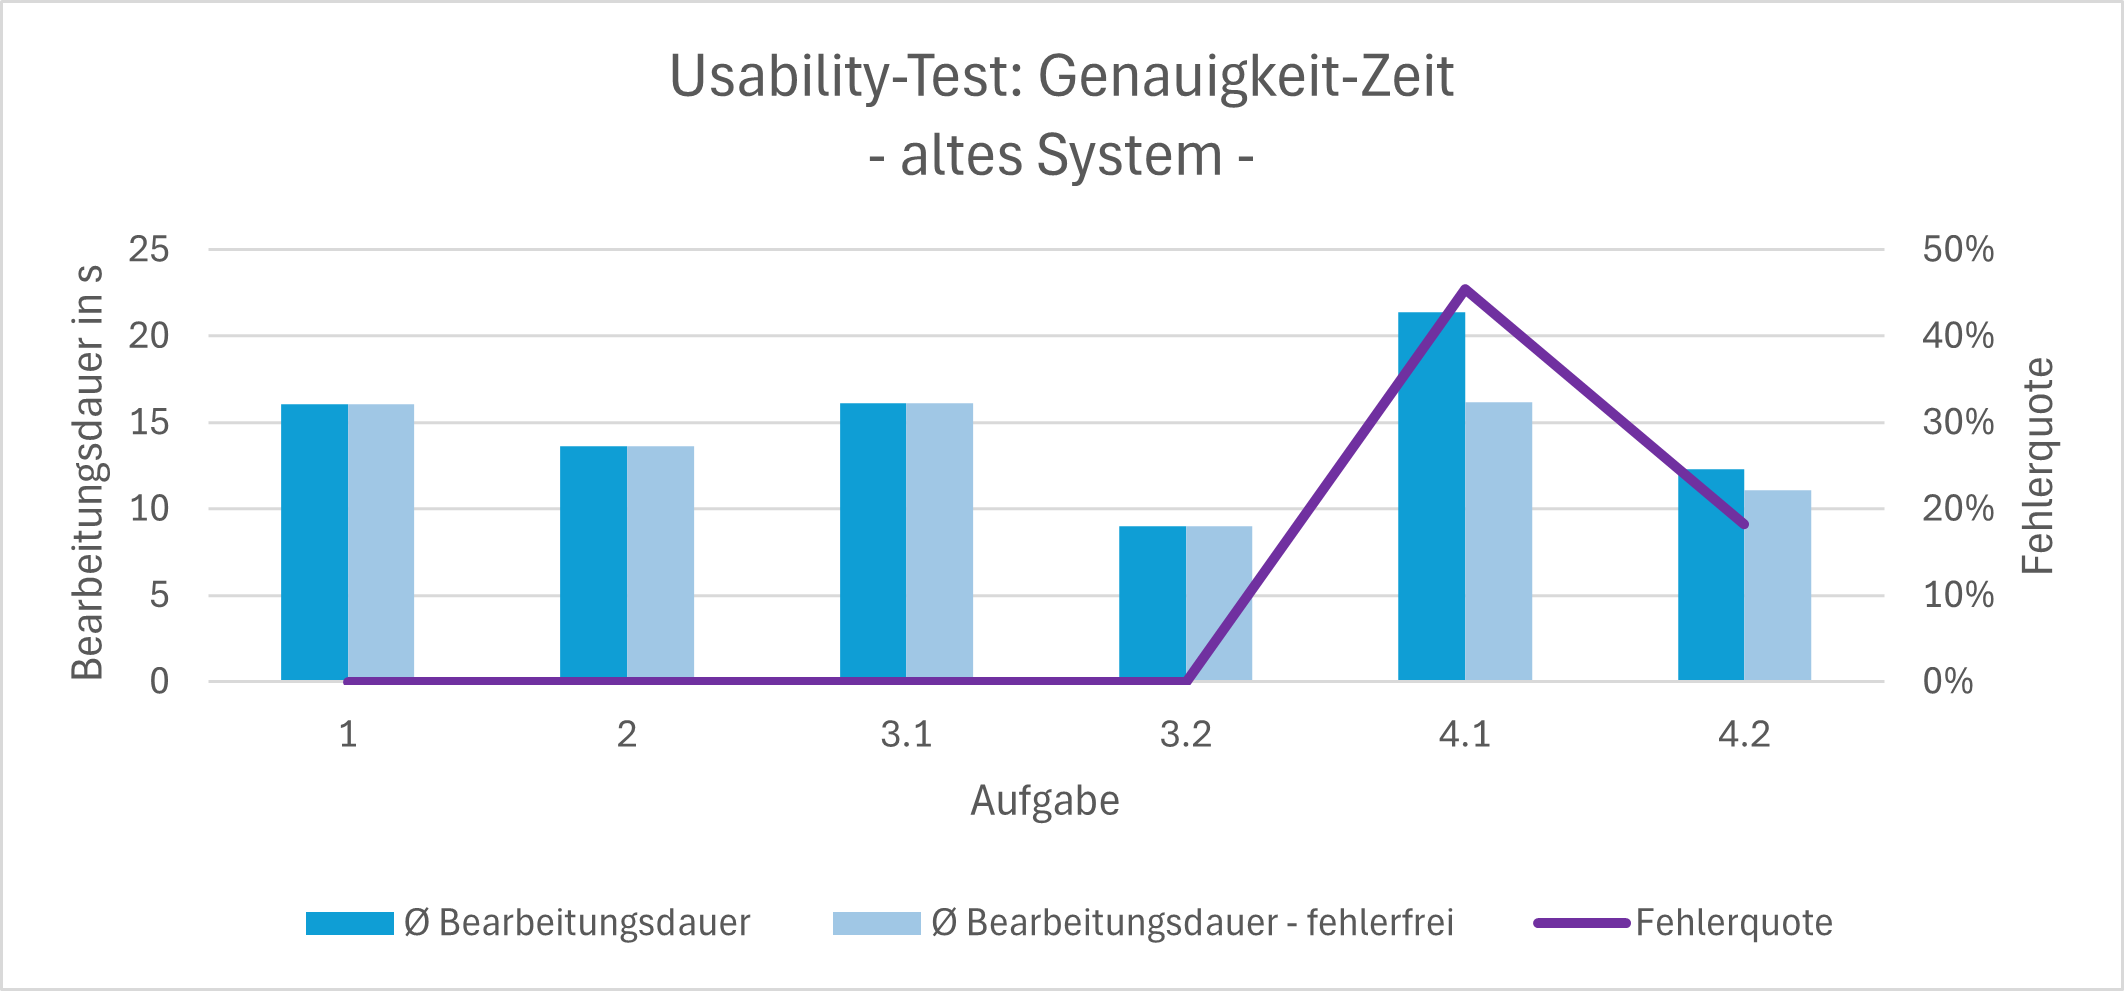
\includegraphics[width=0.8\linewidth]{Diagramme/usability_genauigkeit-zeit_alt.png}
    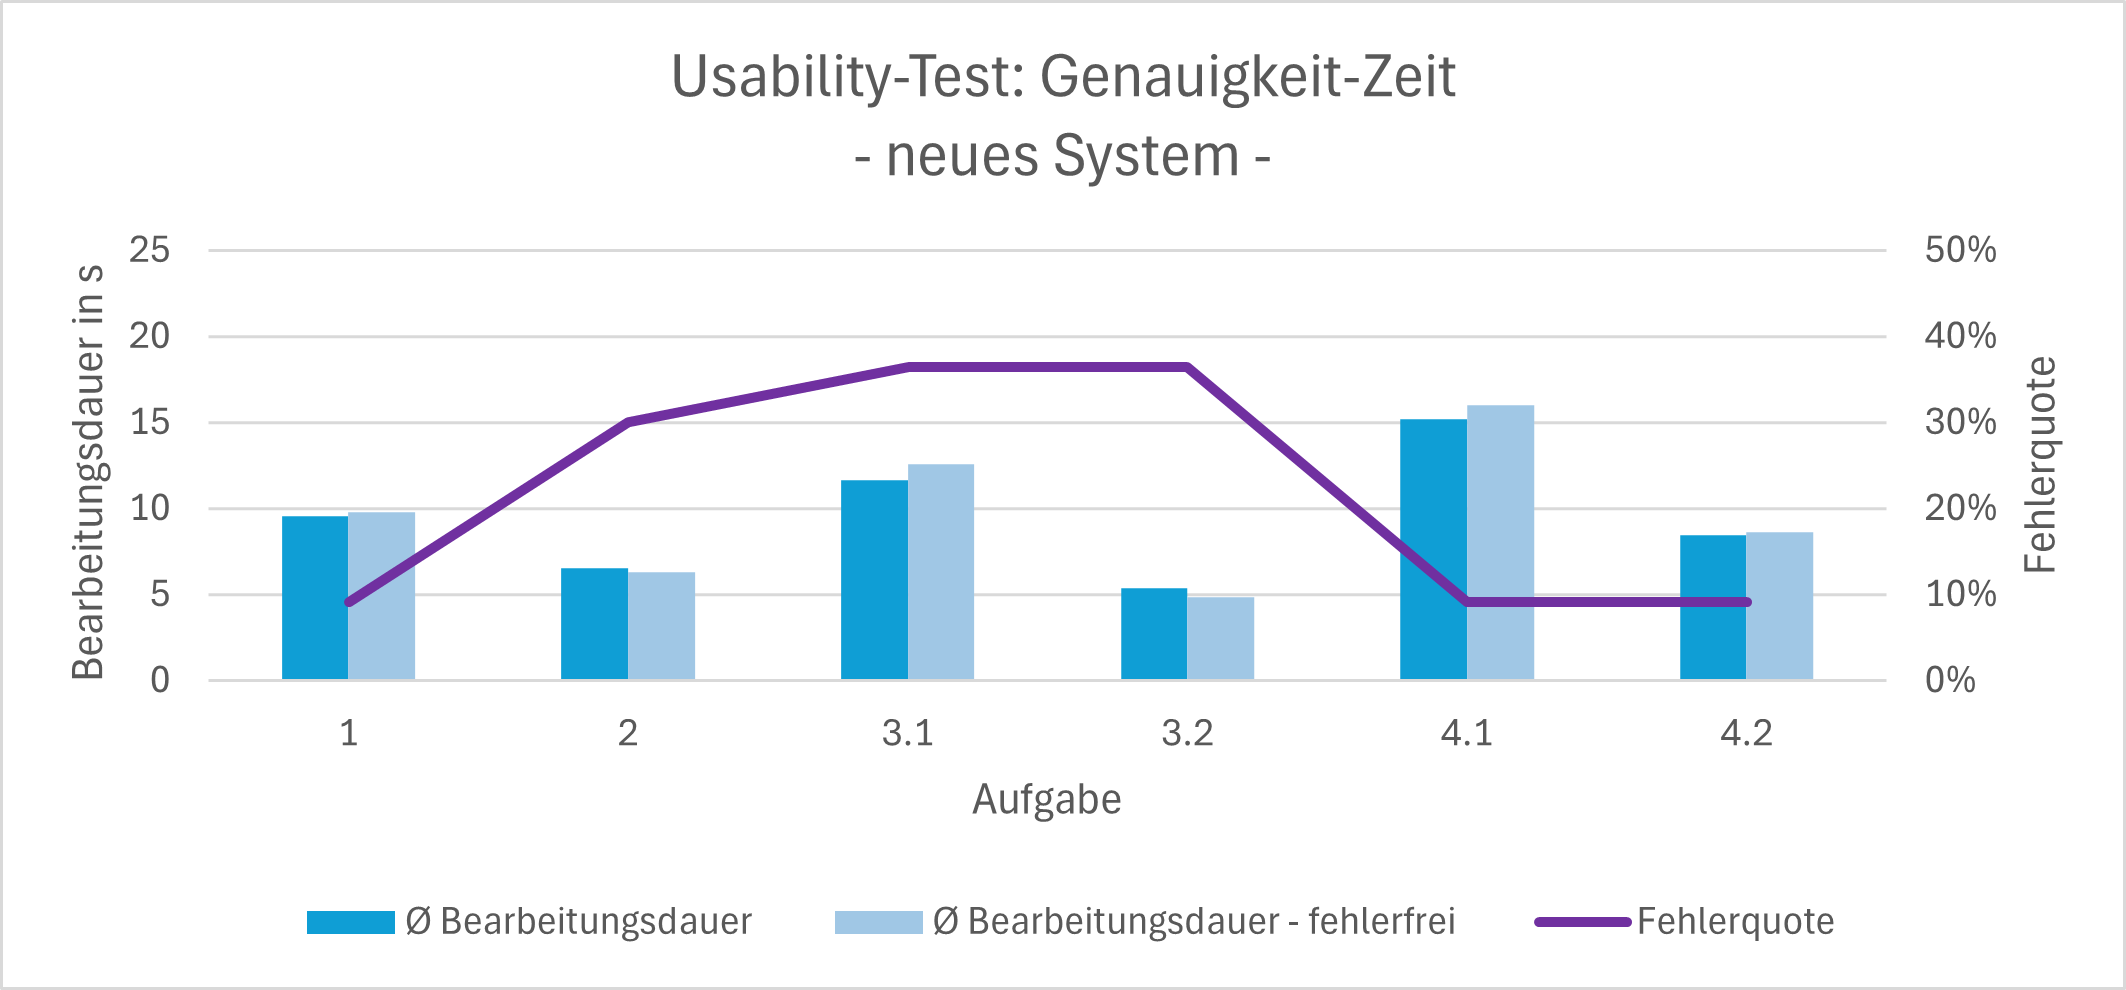
\includegraphics[width=0.8\linewidth]{Diagramme/usability_genauigkeit-zeit_neu.png}
    \caption{Usability-Test: Vergleich Genauigkeit-Zeit im alten und neuen System}
    \label{fig:usability_test:genauigkeit-zeit_alt-neu}
\end{figure}

\noindent
\underline{s. \autoref{fig:usability_test:genauigkeit-zeit_alt-neu}}\\
- alt: Leute mit Fehlern waren langsamer\\
- neu: Leute ohne Fehler waren minimal langsamer, kein signifikanter Unterschied\\
- neu: höhere Fehlerquote, dafür auch x\% schneller (Bsp. Frage 1: 15s auf 10s)\\
-> bei Diskussion darauf eingehen, woher die höhere Fehlerquote kommt

\begin{figure}[H]
    \centering
    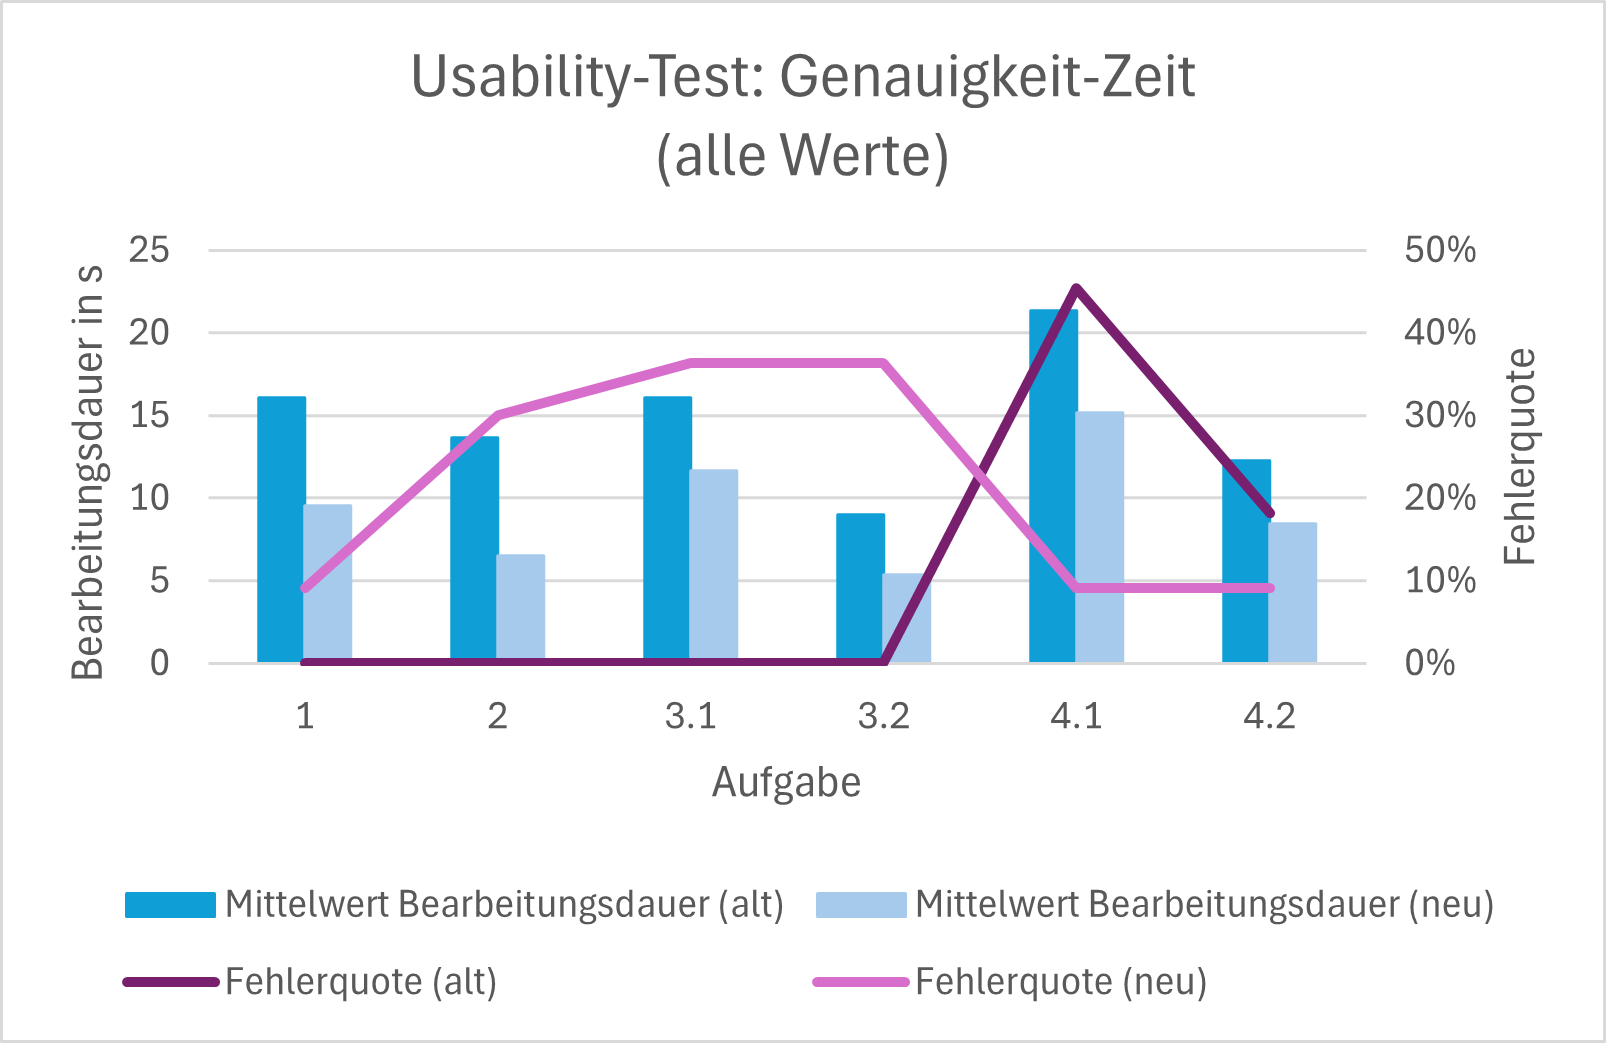
\includegraphics[width=0.8\linewidth]{Diagramme/usability_genauigkeit-zeit_alle.png}
    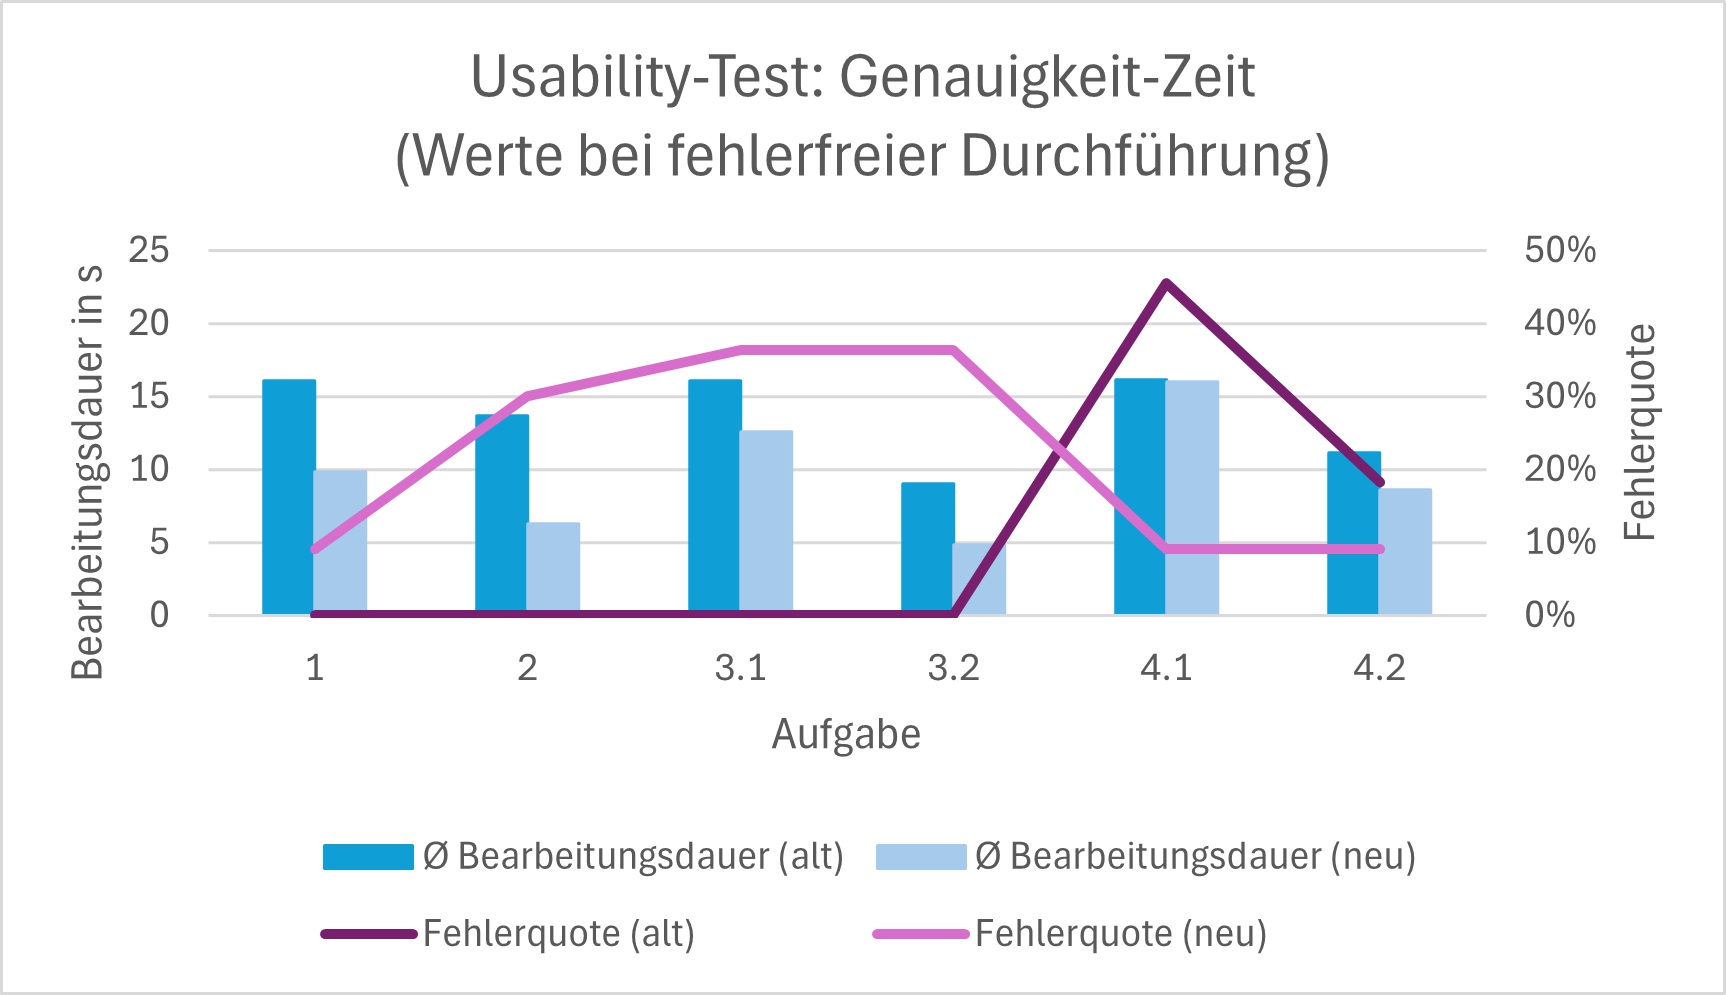
\includegraphics[width=0.8\linewidth]{Diagramme/usability_genauigkeit-zeit_richtige.png}
    \caption{Usability-Test: Zeitvergleich von allen Werten und nur richtigen Antworten - im Verhältnis zur Fehlerquote}
    \label{fig:usability_test:genauigkeit-zeit_alle-richtige}
\end{figure}

\noindent
\underline{s. \autoref{fig:usability_test:genauigkeit-zeit_alle-richtige}}\\
- neu ist in jeder Aufgabe ersichtlich schneller\\
-> Frage nach signifikanz\\
- Fehlerquote nicht überall eindeutig\\

% ****************************************************************************************
\newpage

\noindent
\underline{Statistische Auswertung der Signifikanz}\\
\label{Bsp:ttest}
\label{Beispielrechnung:TTest}
- t-Test Beispielrechnung (einseitig, gepaart)\\
-> erster t-Test zum Verständnis\\
-> erst Normalverteiltes Ergebnis\cite{normalverteilung_rechner}\\
-> die Beispielrechnung gehört in den Text \cite{Statistik:Boertz:2010} \cite{Statistik:Sedlmeier:2024}\\
- Tabelle mit t-Test-Ergebnissen \autoref{tab:usability_test:Differenz+ttest}\\
-> Rest: verweisen auf Ergebnisse aus Excel: $=TTEST(Matrix_{alt}, Matrix_{neu},1,1)$ (s. \autoref{fig:Usability-Test:Excel_Berechnungen})

\noindent
Was macht der T-Test?\\
- Differenzen bilden\\
- davon Mittelwert und Standardfehler berechnen\\
- Aussage treffen, wie wahrscheinlich es ist, dass dieses Ergebnis zufällig entstanden ist\\

\noindent
\begin{table}[H]
Daten: (Frage 1 aus \autoref{fig:pruemper_all})\\
\begin{tabular}{|l|c|c|c|c|c|c|c|c|c|c|c|}
    \hline
    alt         &  2 & 2 & 1 & -1 & 1 & -2 & 2 & -3 & -2 & -1 & -1 \\ \hline
    neu         &  0 & 3 & 1 &  2 & 2 &  1 & 3 &  3 &  3 &  1 & -2 \\ \hline
    \hline
    Differenz x  & -2 & 1 & 0 &  3 & 1 &  3 & 1 &  6 &  5 &  2 & -1 \\
    \hline
\end{tabular}
\end{table}
% TODO: Beispiel aus Prümper, aber Kapitel = Usability-Test

\noindent
Differenzen mit Ergebnis = 0 werden nicht betrachtet \textcolor{red}{TODO: Quelle!}\\
Hypothesen:\\
\textcolor{red}{
$H0:= alt \geq neu$\\
$H1:= alt < neu$\\
}

\noindent
Vorraussetzungen:
\begin{itemize}
    \item 2 abhängige Stichproben
    \item Daten sind metrisch
    \item Differenzen sind normalverteilt
\end{itemize}

\noindent
Anzahl der Fälle:

$\displaystyle n = 10$ \\

\noindent
Freiheitsgrade:

$\displaystyle d_f = n-1 = 9$  \\

\noindent
Mittelwert:
\begin{flalign*}
\indent
\displaystyle
\Bar{x}   &= \frac{\sum{x_{diff}}}{n} &\\
          &= \underline{\underline{1,9}} &\\
\end{flalign*}

\newpage
\noindent
Standardabweichung:
%\newcommand{\thatsum}{ \Xsum\limits_{i=0}^n (i_n - \Bar{x})^2 }
%$$\thatsum$$
\begin{flalign*}
\indent
\displaystyle
    s %&= \sqrt{ \frac{ \Xsum\limits_{i=0}^n (i_n - \Bar{x})^2  }{ n-1 } } &\\
    &= 
    \sqrt
    {
        \frac
        {
            \Xsum\limits_{i=0}^n (i_n - \Bar{x})^2
            % \Xsum_{i=0}^n (i_n - \Bar{x})^2
        }
        {
            n-1
        }
    }&\\
%    =%&=
%    \sqrt
%    {
%        \frac
%        {
%            (x_1 - \Bar{x})^2 +
%            (x_2 - \Bar{x})^2 +
%            (x_3 - \Bar{x})^2 +
%            ... +
%            (x_n - \Bar{x})^2
%        }
%        {
%            n-1
%        }
%    } &\\
    &=
    \sqrt
    {
        \dfrac
        {
            \splitdfrac{
                (-2 - 1,9)^2
                + ( 1 - 1,9)^2
                + ( 3 - 1,9)^2
                + ( 1 - 1,9)^2
                + ( 3 - 1,9)^2
            }{
                + ( 1 - 1,9)^2
                + ( 6 - 1,9)^2
                + ( 5 - 1,9)^2
                + ( 2 - 1,9)^2
                + (-1 - 1,9)^2
            }
        }
        {
            10 - 1
        }
    } &\\
    &=
    \sqrt
    {
        \dfrac
        {
            \splitdfrac{
                (-3,9)^2
                + (-0,9)^2
                + 1,1^2
                + (-0,9)^2
                + 1,1^2
            }{
                + (-0,9)^2
                + 4,1^2
                + 3,1^2
                + 0,1^2
                + (-2,9)^2
            }
        }
        {
            10 - 1
        }
    } &\\
    &=
    \sqrt
    {
        \dfrac
        {
            \splitdfrac{
                15,21
                + 0,81
                + 1,21
                + 0,81
                + 1,21
            }{
                + 0,81
                + 16,81
                + 9,61
                + 0,01
                + 8,41
            }
        }
        {
            9
        }
    } &\\
    &= \sqrt{\frac{54,9}{3}} = \sqrt{6,1} \approx \underline{\underline{2,4698}}
\end{flalign*}

\noindent
Standardfehler des Mittelwerts:\\

$ \displaystyle
s_e = \frac{s}{\sqrt{n}}
    = \frac{2,4698}{\sqrt{10}}
    \approx \underline{\underline{0,7810}}
$\\

\noindent
Teststatistik:\\

$ \displaystyle
t  = \frac{\Bar{x} - 0}{s_e}
   = \frac{\Bar{x}}{s_e}
   = \frac{1,9}{0,781}
   \approx \underline{\underline{2,432778}}
$\\

\noindent
Wahrscheinlichkeit: \textcolor{red}{TODO: Verweis auf die Statistik-Tabelle}\\

$ \displaystyle
p \approx \underline{\underline{0,019471718}}
$ (aus Excel)\\

\newpage
% ****************************************************************************************

\noindent
- Zeiten sind im neuen System in Aufgaben 1+2 signifikant besser als im alten System\\
-> beim Rest nur besser, nicht signifikant\\
- endgültiger Zeitvergleich, s. Zusammenfassung \autoref{fig:usability_test:genauigkeit-zeit_mittel}

\begin{figure}[H]
    \centering
    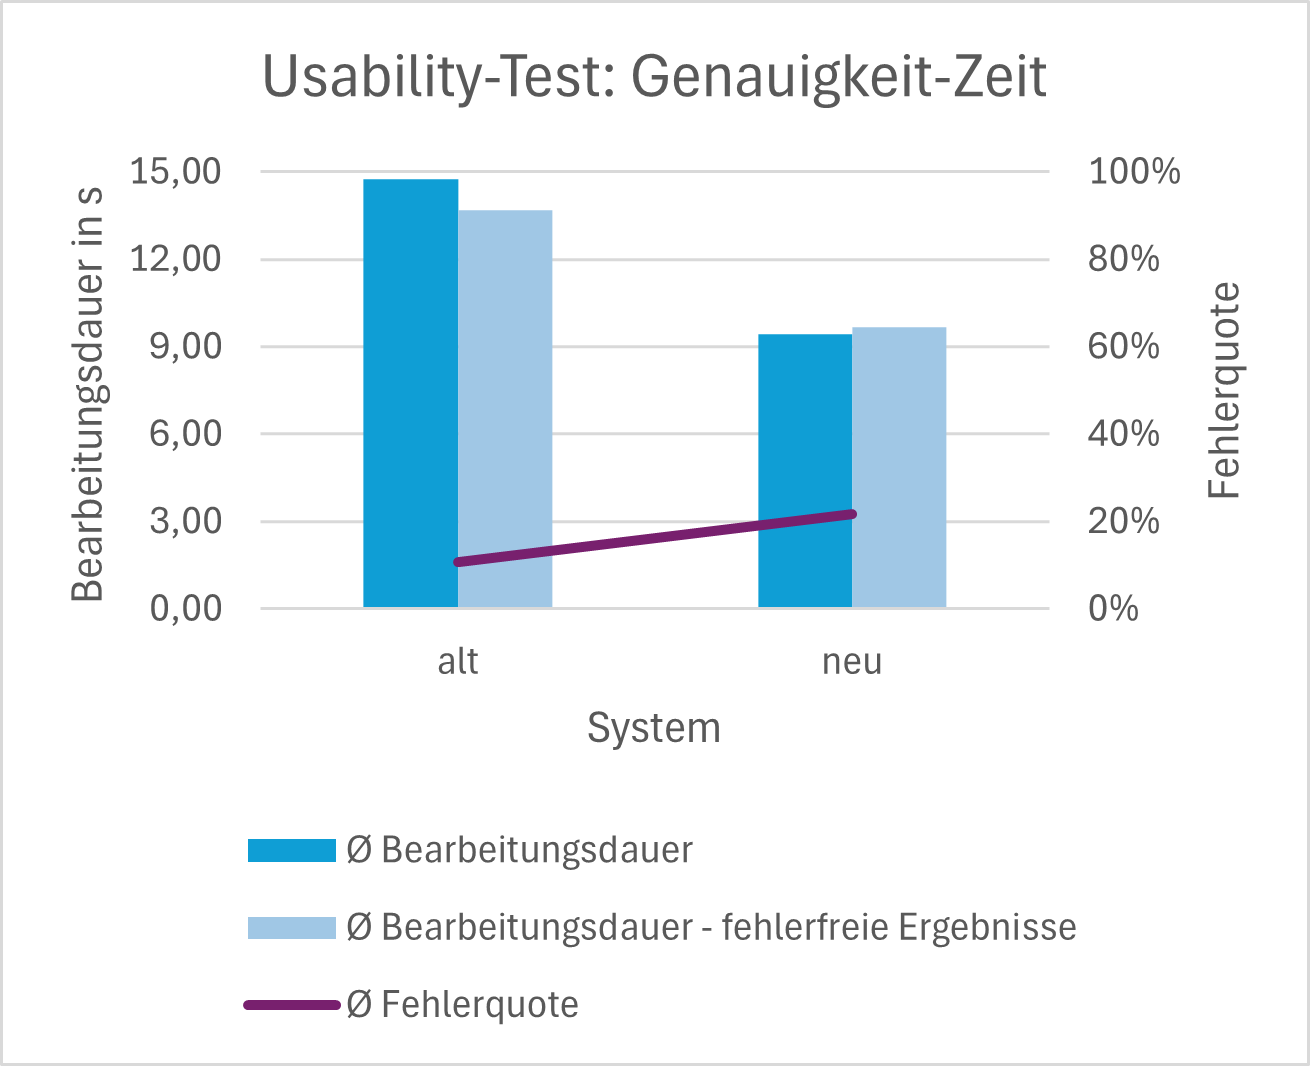
\includegraphics[width=0.8\linewidth]{Diagramme/usability_genauigkeit-zeit_mittel.png}
    \caption{Usability-Test: Vergleich der mittleren Bearbeitungsdauer - im Verhältnis zur Fehlerquote \textcolor{red}{Wo kommen die Daten her?}}
    \label{fig:usability_test:genauigkeit-zeit_mittel}
\end{figure}

\noindent
=> \ref{fig:usability_test:genauigkeit-zeit_mittel} erst in Diskussionskapitel(?)\\
- neu ist im Mittel schneller\\
- aber auch Fehlerquote bei neu im MIttel höher\\
- schöne Zusammenfassung (man kann auch darauf vorspringen)

